\documentclass[a4paper]{article}

\usepackage{fullpage} % Package to use full page
\usepackage{parskip} % Package to tweak paragraph skipping
\usepackage{tikz} % Package for drawing
\usepackage{amsmath}
\usepackage{hyperref}

\title{MTH 4300: Algorithms, Computers, and Programming II}
\author{Fall 2024}
\date{Midterm 2 Review}

\begin{document}
\maketitle


\section{TRUE OR FALSE}
\begin{enumerate}
    \item  Returning by reference allows you to avoid copying an object, 
           improving performance, but returning by value ensures the caller
           receives a new copy of the object.
    \item The this pointer in C++ is a constant pointer that holds the address
          of the current object.
    \item The size of an std::vector is fixed once it is created and cannot change.
    \item std::list in C++ allows random access to its elements, just like std::vector.
    \item You can overload the arrow (->) operator in a class, and it is commonly
          used when a class contains or behaves like a pointer.
    \item In a singly linked list, each node has a pointer to the previous node as well as the next node.
    \item The time complexity of the selection sort algorithm is O(n log n) in the worst case.
    \item The fstream class in C++ allows for both input and output operations on files.
    \item Overloaded operators must have at least one operand that is of user-defined type.
    \item In C++, using header guards (or #pragma once) is essential in 
          multifile projects to prevent multiple inclusions of the same header file.
\end{enumerate}
\newpage


\section{SHORT ANSWER}
\begin{enumerate}
    \item Name 
\end{enumerate}
\newpage 


\section{CODING}
\begin{enumerate}
    \item 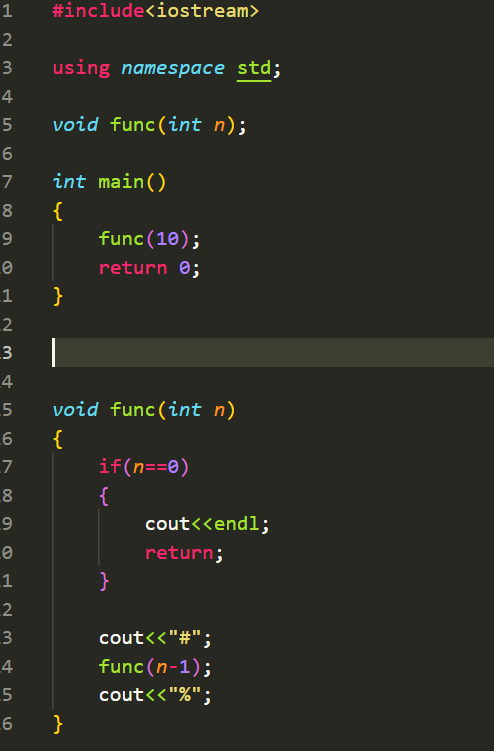
\includegraphics[width=5cm]{question2.png}
    
\end{enumerate} 
\newpage

\section{SOLUTIONS}
\subsection{TRUE OR FALSE}
\begin{enumerate}
    \item true
    \item true
    \item \href{run:./coding_question4.cpp}{coding\_question4.cpp}
\end{enumerate}


\end{document}